\documentclass[12pt]{article}
\usepackage[a4paper, total={7.5in, 11in}]{geometry}
%\usepackage{array}
\usepackage{graphicx, subfig, wrapfig, fancyhdr, lastpage, multicol ,color,arydshln,makecell, mhchem}
\newcommand\headerMe[2]{\noindent{}#1\hfill#2}
\usepackage[mathscr]{euscript}
\usepackage{tabularray}

\setlength{\columnseprule}{1pt}
\def\columnseprulecolor{\color{blue}}


\pagestyle{fancy}
\fancyhf{}

\cfoot{ \vspace{-0.8cm}\em{Page \thepage \hspace{1pt} / \pageref{LastPage}}}
\begin{document}

\headerMe{Royaume du Maroc}{année scolaire \emph{2024-2025}}\\
\headerMe{Ministère de l'Éducation nationale, }{  Professeur :\emph{Zakaria Haouzan}}\\
\headerMe{du Préscolaire et des Sports}{Établissement : \emph{Lycée SKHOR qualifiant}}\\
\vspace{-1cm}
\begin{center}
Devoir Surveillé  N°2 \\
    2ème année baccalauréat Sciences physiques\\
Semestre 2 - Durée 1h30
\\
    \vspace{.2cm}
\hrulefill
\Large{Chimie 7pts - 35min}
\hrulefill\\

    %\emph{Les deux parties sont indépendantes}
\end{center}
%end Headerss------------------------
%__________________Chimie ______________________-
%%%%%%%+_+_+_+_+_+_+_+_+_Partie1
%\vspace{-1cm}
 \section*{Exercice 1 :Transformations spontanées dans les piles et récupération de
l’énergie. \dotfill(7pts) }
\begin{wrapfigure}[1]{r}{0.3\textwidth}
	\vspace{-1.2cm}
\begin{center}
  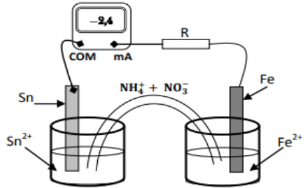
\includegraphics[width=0.3\textwidth]{./ex_00.png}
\end{center}
\end{wrapfigure}

on réalise la pile suivante avec : $S_1$ solution de sulfate d'étain(II) \\$(Sn^{2+} + SO_4^{2-})$ de concentration $C_1$=$0.5mol/L$ et $V_1=200mL$.
et  $S_2$ \\solution de sulfate de cuivre(II) $(Fe^{2+} + SO_4^{2-}$) de concentration $C_2=0.2mol/L$ \\et $V_2=200mL$. un pont salin .

on donne : $1F=96500 C/mol$ , $M(Fe)=56g/mol$

\begin{tabular}{c|l}
	0,5  & \makecell[l]{ \textbf{1. }Indiquer sur le schéma le sens du déplacement des porteurs \\de
charges.}\\
	1  & \makecell[l]{ \textbf{2. }Quel est le rôle du pont salin? }\\
	0,5  & \makecell[l]{ \textbf{3. }Donner le schéma conventionnel de la pile étudiée. }\\
	1 & \makecell[l]{ \textbf{4. }Indiquer la cathode et l’anode avec \underline{justification}}\\ 
	1 & \makecell[l]{ \textbf{5. }Ecrire les demi-équations et l’équation qui modélise le
fonctionnement de la pile}\\
	1	& \makecell[l]{ \textbf{6. }Calculer le temps de fonctionnement maximal de la pile pour une
intensité \\constante $I_0=0.5 A$.}\\
		2 & \makecell[l]{ \textbf{7. }On change l’intensité I et on remarque que la masse de l’électrode de fer a diminuée \\de $28mg$ pendant un
		fonctionnement de $1h15min$, \underline{calculer l’intensité I} }\\
	\end{tabular}

%\hrulefill
%\Large{Physique 13pts/78min}
%\hrulefill\\
\begin{center}
    %\vspace{.60cm}
\hrulefill
\Large{Physique 13pts - 55min}
\hrulefill\\
    \emph{Les  parties sont indépendantes}
\end{center}

\vspace{-1cm}


	\section*{Partie 1 : l’énergie E emmagasinée par la bobine \dotfill(5,5pts)}

\begin{wrapfigure}[9]{r}{0.25\textwidth}
  \begin{center}
	  \vspace{-1cm}
	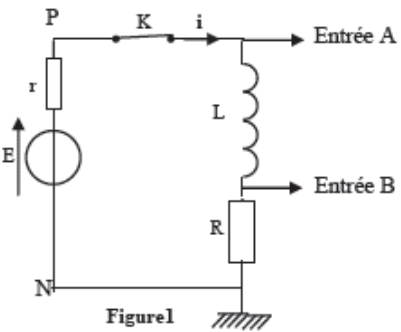
\includegraphics[width=0.22\textwidth]{./img/img03.png}
	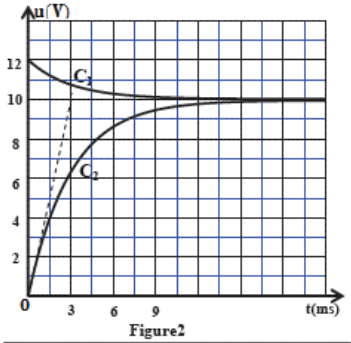
\includegraphics[width=0.25\textwidth]{./img/img04.png}
  \end{center}
\end{wrapfigure}
On réalise le circuit électrique, schématisé sur la figure 1, qui comporte : 
	\begin{itemize}
		\item  Un générateur de tension de f.e.m. $E=12V$
		\item  Une bobine d’inductance L et de résistance négligeable ;
		\item  Deux conducteurs ohmiques de résistance $R = 40\Omega$
		\item  Un interrupteur K.

	\end{itemize}

On ferme l’interrupteur K à l’instant $t=0$. Avec un système d’acquisition informatisé, on enregistre les
courbes (C2) et (C1 ) représentant les tensions des voies A et B (voir figure2).

\begin{tabular}{c|l}	

	0,25 & \makecell[l]{\textbf{1. }Identifier la courbe qui représente la tension $u_R (t)$ et celle qui\\représente $u_{PN} (t)$.}\\
	0,25 & \makecell[l]{\textbf{2. }Vérifier que la valeur de la résistance $r$ du conducteur ohmique  \\est $r=8\Omega$. }\\
	
	1 & \makecell[l]{\textbf{3. }Etablir l’équation différentielle régissant l’établissement du courant $i(t)$ dans le circuit.  }\\
	1 & \makecell[l]{\textbf{4. }Trouver les expressions de A et de $\tau$ en
fonction des paramètres du circuit pour
que \\l’expression $i(t) =A (1-e^{-\frac{t}{\tau}} )$, soit solution de
cette équation différentielle. }\\

	1 & \makecell[l]{\textbf{5. }Déterminer la valeur de la constante du temps $\tau$. }\\
	1 & \makecell[l]{\textbf{6. }En déduire la valeur de l’inductance L de la bobine. }\\
	1 & \makecell[l]{\textbf{7. }Trouver l’énergie E emmagasinée par la bobine à l’instant $t = \frac{\tau}{2}$. }\\
\end{tabular}





\section*{Partie 2 :  Circuit RLC série. \dotfill(2.25pts)}
\vspace{-0.4cm}

\begin{wrapfigure}[1]{r}{0.25\textwidth}
	\vspace{-1.2cm}
\begin{center}
  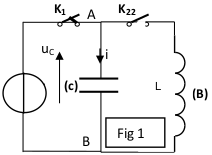
\includegraphics[width=0.25\textwidth]{./ex_011.png}
\end{center}
\end{wrapfigure}


On considère le circuit électrique schématisé dans la figure 4, comportant :

\begin{itemize}
	\item Un générateur de tension continue (G), de f.é.m $U_0$ et de résistance interne \\ négligeable, Un condensateur (c) de capacité C et d’armatures A et B ;
	\item Une bobine (B) d’inductance L et de résistance négligeable ;
	\item Deux interrupteurs $K_1$ et $K_2$.

\end{itemize}

Le condensateur étant chargé, à t = 0 on ouvre $K_1$ et on ferme $K_2$. A t quelconque, l’armature A du
condensateur porte une charge q.

\begin{tabular}{c|l}

	0,5 & \makecell[l]{\textbf{1. }Etablir l’équation différentielle des oscillations électriques.  }\\
	
	0,25 & \makecell[l]{\textbf{2. }Déterminer l’expression de la période propre $T_0$ en fonction de L et C.  }\\

	0,5 & \makecell[l]{\textbf{3. }Donner l’expression de l’énergie magnétique $E_L$ en fonction de L et i }\\

	1 & \makecell[l]{\textbf{4. }Montrer que l’expression de cette énergie $E_L$ en fonction du temps s’écrit :   \\\hspace{3cm}$E_L = \frac{E_0}{2}.\bigg(1+cos\big(\frac{4.\pi}{T_0}.t + \pi \big)\bigg) $ }\\
\end{tabular}



\section*{Partie 2 :  Applications: Production d'ondes électromagnétiques et
communication \dotfill(5.25pts)}

\begin{wrapfigure}[1]{r}{0.3\textwidth}
	\vspace{-1.2cm}
\begin{center}
  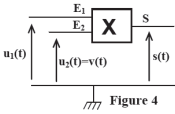
\includegraphics[width=0.3\textwidth]{./ex_033.png}
\end{center}
\end{wrapfigure}



Le circuit de modulation est constitué d’un composant nommé multiplieur
qui possède deux entrées E1 et E2 et une sortie S,

Pour simuler la modulation d’amplitude, on applique :
\begin{itemize}

	\item À l’entrée $E_1$ le signal $u_1(t)=u(t)+U_0$ dont $u(t)=U_mcos(2.\pi.f.t)$ est\\ le
signal modulant et $U_0$ tension continue de décalage .
\item À l’entrée $E_2$ le signal porteur $u_2(t)=v(t)=V_m.cos(2.\pi.F.t)$.
\item Le circuit intégré X donne une tension modulée proportionnelle
au produit des deux tensions, $s(t)$=$ k.u_1(t).u_2(t)$ où k est une
constante dépendant uniquement du circuit intégré . s(t) s’écrit
sous la forme : $s(t)$=$S_mcos(2.\pi.F.t)$.
\end{itemize}

\begin{wrapfigure}[1]{r}{0.3\textwidth}
	\vspace{-3.5cm}

\begin{center}
  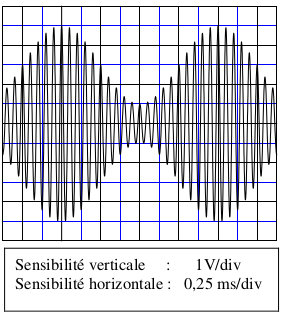
\includegraphics[width=0.3\textwidth]{./ex_034.png}
\end{center}
\end{wrapfigure}


\begin{tabular}{c|l}
	0,5 & \makecell[l]{\textbf{2.1. }Montrer que $S_m$,amplitude du signal modulé , peut se
mettre sous la forme\\ $S_m = A.\big[m.cos(2.\pi.f.t)+1\big]$ en précisant
l’expression du taux de modulation m et celle de la \\constante A . }\\
		&\makecell[l]{\textbf{2.2. }Le graphe représenté sur la figure (5) donne l’allure de la
tension modulée en fonction \\du temps. Déterminer à partir de ce
graphe : }\\
		0,25& \makecell[l]{\textbf{2.2.1. }la fréquence F de l’onde porteuse .}\\
		0,25& \makecell[l]{\textbf{2.2.2. }la fréquence $f$ de l’onde modulant .}\\
		0,25& \makecell[l]{\textbf{2.2.3. }L’amplitude minimale $S_{m(min)}$ et l’amplitude maximale \\$S_{m(max)}$ du signal modulé.}\\

		1 &\makecell[l]{\textbf{2.3. }Donner l’expression du taux de modulation en fonction \\de $S_{m(min)}$ et $S_{m(max)}$. Calculer la valeur de m . }\\

	0,5 &\makecell[l]{\textbf{2.4. }La modulation effectuée est-elle de bonne qualité ? \\Justifier. }\\

	2,5 &\makecell[l]{\textbf{2.5. }Pour une bonne réception du signal modulée, on utilise\\ un
circuit bouchon(circuit d'accord) formé d'une bobine
\\d'inductance $L_0 = 60mH$ et de résistance négligeable et
deux \\condensateurs , montés en série, de capacité $C =10\mu.F$
et $C_0$ .\\\underline{Déterminer la valeur de $C_0$?}. Tracer le disjoncteur (circuit d'accord) et \\expliquer le rôle de chaque étape ? }

\end{tabular}

\end{document}
